The challenge in any text-based modeling approach is the representation of data. A computer cannot comprehend words like humans, thus it needs a numeric approach for text analysis. This leads to the idea of using ids to map words~\parencite{nlpfundamentals}. For example, consider the sentence: “John went to the park.”. We can easily construct a basic dictionary for the words in this sentence and map them to a unique id as such: 

$\{"john" : 0, "went" : 1, "to" : 2, "the" : 3, "park" : 4\}$

\subsubsection{One-Hot Encoding}
This process could also occur for categories that need to be numerically represented, such as publications. However, this map tells the model that “park” is more important, or weighted more heavily, than “john”. If the model calculates averages, it will find the average of the words “went” and “the” to equal “to”. These types of relationships are incorrect and would inhibit the model’s effectiveness. To mitigate this problem, researchers developed the concept of one-hot encoding, which binarizes the process of mapping items to their numeric representations~\parencite{harris_harris_2015}. A matrix is generated with dimensions (length of items in entry X length of total dictionary) for each example. Each row of the matrix has a single one and all other entries are zero to represent the single word. Using the above example, our sentence representation would become:

\[\begin{bmatrix}
1 & 0 & 0 & 0 & 0\\
0 & 1 & 0 & 0 & 0\\
0 & 0 & 1 & 0 & 0\\
0 & 0 & 0 & 1 & 0\\
0 & 0 & 0 & 0 & 1\\
\end{bmatrix}\]

Although this solves the initial problem, there are some disadvantages to this approach. Firstly, the creation of such sparse matrices for each entry in a large dataset is inefficient for storage purposes. It is also plagued by the “curse of dimensionality” as each category appends an entire dimension to the matrix~\parencite{bellman_1954}. The addition of items to the dictionary leads to changing the representations for all previous words. 

This approach also lacks interpretability. As the items are fed into the model, the one-hot encoded matrix tells the user nothing about the relationship between words. It also breaks down word order, which is required for models such as \acrshort{bert}.

\subsubsection{Embedding Vectors}
These problems led to the development of vectorized word representations (embeddings). Word embeddings map each word to a unique n-sized vector of a single dimension. The embeddings are not directly interpretable by humans, as they capture latent qualities of the word, however embeddings offer a significant advantage over alternatives in their ability to offer comprehensible representations. Similar words will be found to be spatially contiguous. The relationship between words can also be calculated directly through cosine similarity~\parencite{dot_products_2008}. The most famous example of this type of interpretability is the mathematical relationship \textbf{king - man + woman = queen} which can be observed in \Cref{fig:king_man_woman_queen_pic}.

\begin{figure}[h]
\centering
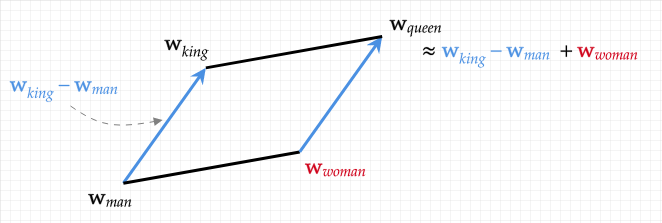
\includegraphics[width=0.8\textwidth]{fig/king-man-woman-queen.png}
\caption{Spatial representation of king - man + woman = queen~\textcite{king_man_woman_queen}}
\label{fig:king_man_woman_queen_pic}
\end{figure}

This allows for each example in the dataset to be represented as a unidimensional list of word ids, which can be mapped to their corresponding vectors when being processed by the model. The data storage advantages are obvious, as each entry becomes easily stored as a single dense list instead of a highly-sparse matrix. Cecause of both the data-related and interpretability advantages offered by embeddings, they were utilized for both of the tested models.